\documentclass[10pt,conference]{IEEEtran}
%\IEEEoverridecommandlockouts
\usepackage[spanish,es-tabla]{babel}
\usepackage[spanish]{babel}
\renewcommand{\baselinestretch}{1.5}     %interlineado
\usepackage[utf8]{inputenc} 
\usepackage[square,numbers]{natbib}
\bibliographystyle{abbrvnat}
\usepackage{float}                      % para usar [H]
\usepackage{amsmath,amssymb,amsfonts}
\usepackage{graphicx}
\usepackage{textcomp}
\usepackage{xcolor}
\usepackage{ragged2e} % \justify

%---------- encabezado pagina
\usepackage{fancyhdr}
\pagestyle{fancy}
\fancyhf{}
\rhead{\thepage}
\renewcommand{\headrulewidth}{0pt}
%-----------------


%-----------------
\def\BibTeX{{\rm B\kern-.05em{\sc i\kern-.025em b}\kern-.08em
    T\kern-.1667em\lower.7ex\hbox{E}\kern-.125emX}}
%__________

\title{Redes Bayesianas \\ {\Large Inteligencia Artificial 2}}
%--------------------------------------------
\author{
\IEEEauthorblockN{1\textsuperscript{do} Angely Mendez}
\IEEEauthorblockA{\textit{Escuela de Informática} \\
\textit{Universidad Nacional de Trujillo}\\
Trujillo, Perú \\
t052701020@unitru.edu.pe}
\and
\IEEEauthorblockN{2\textsuperscript{ero} Ciara Mendez}
\IEEEauthorblockA{\textit{Escuela de Informática} \\
\textit{Universidad Nacional de Trujillo}\\
Trujillo, Perú \\
t022700920@unitru.edu.pe}
}

%%--------------------------------------------
\begin{document}
\renewcommand{\IEEEkeywordsname}{{\bfseries Palabras claves:}} % Colocar Keywords en Spanish

\maketitle
%-------------------------------------------
\begin{abstract}
Este documento es una investigación que describe las Redes Bayesianas. Este articulo es la recopilación de varias investigaciones a nivel nacional e internacional, en los que abordan un problema y resultados, estas redes bayesianas permiten modelar procesos caracterizados por la incertidumbre, lo cual es propio de muchos problemas reales. Con una red bayesiana se puede establecer un modelo completo sobre un conjunto de variables aleatorias y sus relaciones y empleados correctamente hacen que un programa exhiba un comportamiento inteligente; respecto a las Redes Bayesianas, se explica su definición y cuatro investigaciones sobre ellas, con la finalidad de entender la importancia de las ciencias de la computación en la vida diaria.  
\end{abstract}

\begin{IEEEkeywords}
Redes Bayesianas, Probabilidad, ciencias de la computación, inteligencia artificial.
\end{IEEEkeywords}

\section{\textbf{Introducción}}
Es de suma importancia las relaciones de independencia y de independencia condicional en la simplificación de las representaciones probabilistas del mundo. Por ello, un modo sistemático para representar explícitamente tales relaciones es la forma de Redes Bayesianas.\par
La sintaxis y semántica de estas redes pueden utilizarse para capturar conocimiento incierto de un modo natural y eficiente. Además, la inferencia probabilista, aunque computacionalmente intratable en el peor de los casos, puede hacerse eficiente en muchas situaciones prácticas.\par
Entonces este informe presenta información al respecto, el cual está organizado de la siguiente manera: en primer lugar, se explican los conceptos teóricos: definición de las redes bayesianas y como está conformada, luego se da énfasis en cuatro investigaciones sobre aplicaciones de este tema y para finalizar las conclusiones más relevantes.
%------------------------------------------
\section{\textbf{Redes Bayesianas}} 
%\vspace{-22 mm}
Una red bayesiana es un grafo dirigido en el que cada nodo está comentado con información probabilista cuantitativa \citep{russell2004inteligencia}.

La especificación completa es como sigue:
\begin{enumerate}
    \item Un \textbf{conjunto de variables} aleatorias forman los nodos de la red. Las variables pueden ser discretas o continuas.
    \item Un \textbf{conjunto de enlaces dirigidos} o flechas conectan pares de nodos. Si hay una flecha de un nodo X a un nodo Y, se dice que X es un padre de Y.
    \item Cada nodo Xi tiene una \textbf{distribución de probabilidad condicionada} $P(Xi\|Padres(Xi))$ que cuantifica el efecto de los padres del nodo.
    \item El grafo no tiene ciclos dirigidos (y así es un grafo acíclico dirigido, o GAD).  
\end{enumerate}

La topología de la red (el conjunto de nodos y enlaces) (Ver Figura  ~\ref{R1}), especifica las relaciones de independencia condicional que se tienen en el dominio. El significado intuitivo de una flecha en una red construida correctamente es, habitualmente, que X tiene una influencia directa sobre Y.

\begin{figure}[H]
\begin{center}
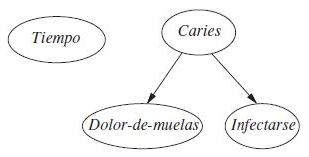
\includegraphics[width=6cm, height=3cm]{figuras/R1.JPG}
\caption{Una red bayesiana sencilla en la que Tiempo es independiente de las otras tres variables y Dolor-de-muelas e Infectarse son independientes condicionalmente, dada Caries.}
\label{R1} 
\end{center}
\end{figure}

Es generalmente sencillo para un \textbf{experto del dominio} decidir qué influencias directas existen en el área, mucho más sencillo, de hecho, que la especificación de las probabilidades. Una vez que la topología de la red bayesiana está diseñada, necesitamos sólo especificar una distribución de probabilidad condicional para cada variable, dados sus padres. Veremos que la combinación de la topología y las distribuciones condicionales son suficientes para especificar (implícitamente) la distribución conjunta completa para todas las variables. 

\begin{figure}[H]
\begin{center}
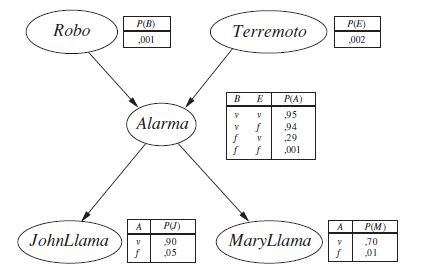
\includegraphics[width=7cm, height=5cm]{figuras/R2.JPG}
\caption{Una red bayesiana típica, mostrando tanto la topología de la red como las tablas de probabilidad condicional (TPCs). En las TPCs, las letras B, E, A, J y M significan Robo, Terremoto, Alarma, JohnLlama y MaryLlama, respectivamente}
\label{R2} 
\end{center}
\end{figure}

En la figura ~\ref{R2}, cada distribución se muestra como una \textbf{tabla de probabilidad condicional, o TPC}. (Este formato de tabla puede usarse para variables discretas; otras representaciones, incluyendo las adecuadas para variables continuas) Cada fila de una TPC contiene la probabilidad condicional de cada valor del nodo para un caso de condicionamiento. Un caso de condicionamiento es una combinación posible de valores de los nodos padres (un suceso atómico en miniatura, si prefiere). Cada fila debe sumar 1, ya que las entradas representan un conjunto exhaustivo de casos para la variable.

De acuerdo a Palma y Roque \citep{morales2011inteligencia}, las redes bayesianas son estructuras gráficas (grafos dirigidos aciclícos) que permiten modelar el conocimiento incierto sobre un conjunto de variables y razonar con él. Constan de dos componentes:

\begin{enumerate}
    \item \textbf{Componente cualitativa}. Definida por el conjunto de variables (nodos) y el conjunto de arcos (o enlaces) que conectan pares de nodos. La topología del grafo representa las dependencias entre variables tanto directas, a través de sus arcos, como también mediante los patrones de conexión estudiados para redes causales. 
    
    \item \textbf{Componente cuantitativa}. La define un conjunto de valores de probabilidad que indican la fuerza de la conexión entre pares de variables enlazadas. Parece natural que, desde la perspectiva probabilística, se considere que la fuerza de un enlace $X → Y$ sea $P(Y\|X)$. Claro que si Y tuviera como padres a X y a Z debería considerarse cómo interactúan los dos sobre Y , por lo que se debería especificar $P(Y\|X,Z).$
\end{enumerate}

A continuación, se presentan cuatro investigaciones donde se evidencia la aplicación de las Redes Bayesianas:
\begin{enumerate}
\item En la investigación \textit{\textbf{“Empleo de las redes bayesianas para apoyar la toma de decisiones sobre la propagación de la Covid-19”}}, \citep{cordero2021empleo}.

\textbf{\underline{Problema:}} Las aplicaciones existentes para apoyar la toma de decisiones sobre la propagación de la Covid-19 son escasas. Generalmente han estado centradas en el uso de modelos matemáticos que utilizan datos discretos en la búsqueda del conocimiento sobre la evolución de la epidemia, considerando a los sujetos susceptibles, expuestos, infectados y recuperados. Los modelos referidos presentan características variables y no son suficientes para solucionar el problema. Hecho que muestra la necesidad de una herramienta de apoyo para el análisis certero de la propagación de la Covid-19, con el fin de obtener un mejor grado de acierto en las propagaciones de la enfermedad y que contribuya apoyar la toma de decisiones, con el fin de disminuir las afectaciones que esta enfermedad provoca.

\textbf{\underline{Resultados:}} La investigación realizó un estudio de las redes bayesianas como una herramienta para resolver distintos problemas en los modelos matemáticos que utilizan datos discretos en la búsqueda del conocimiento sobre la evolución de la epidemia. La Figura ~\ref{RB1}, muestra que la Covid-19, es la enfermedad donde los síntomas con mayor relevancia son: Fiebre y Falta de aire, por lo que los arcos representan una dirección de diagnóstico e introduce información numérica, que corresponde a la tabla de probabilidad condicionada (TPC) de cada nodo, obtenido en base a la experiencia de los médicos. La muestra seleccionada fueron 520 pacientes de diferentes grupos etarios con los síntomas referidos en el periodo de aparición de la Covid-19, en el hospital de la Habana, Cuba.

\begin{figure}[H]
\begin{center}
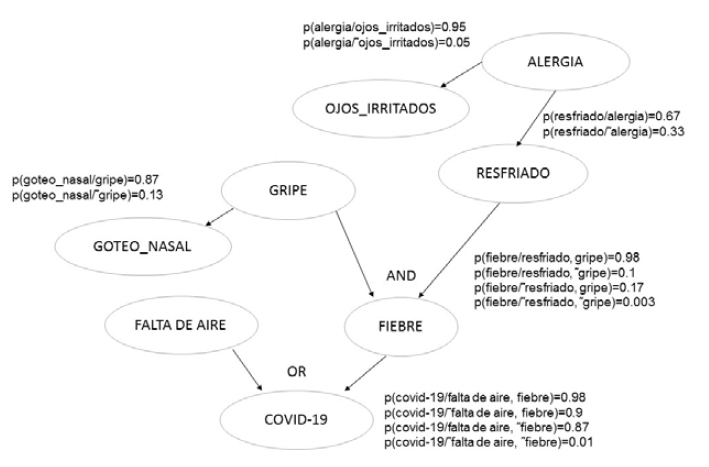
\includegraphics[width=8.5cm, height=6cm]{figuras/RB1.PNG}
\caption{Grafo para apoyar la toma de decisiones sobre la propagación de la Covid-19.}
\label{RB1} 
\end{center}
\end{figure}

\textbf{\underline{Importancia:}} 
Las redes bayesianas proveen información sobre las relaciones de dependencia e independencia condicional existentes entre variables. La inclusión de las relaciones de independencia en la propia estructura de la red, hace de las redes bayesianas una buena herramienta para representar conocimiento de forma compacta y apoyar la toma de decisiones sobre la propagación de la Covid-19, pues reduce el número de parámetros. Además, la posibilidad de trabajar con datos discretos y continuos simultáneamente, y la flexibilidad en la estructura del modelo.

\item Otra investigación es \textit{\textbf{“Las finanzas de los hogares mexicanos: análisis con redes bayesianas”}}, \citep{davila2021finanzas}.

\textbf{\underline{Problema:}}
El bienestar de los hogares está ligado en gran parte al desarrollo de los mercados financieros. El estudio de las finanzas de los hogares analiza las formas en que utilizan instrumentos financieros para satisfacer sus necesidades y objetivos; este análisis es un gran desafío debido a la escasa información estadística y la interrelación entre variables. Enfocado en el caso de México, se pueden seguir dos vertientes: la primera basada en la teoría de las finanzas tradicionales, de decisiones racionales (comportamiento ideal) y los tomadores de decisiones tienen cierto grado de educación financiera y procuran maximizar su beneficio. La segunda, en las finanzas conductuales, las personas no toman las decisiones de manera óptima necesariamente e implica contar con datos reales, que no siempre están disponibles. En esta investigación se pretendió conciliar ambas vertientes aplicando redes bayesianas. 

\textbf{\underline{Resultados:}} En este trabajo, se utilizó de manera conjunta las finanzas tradicionales y las conductuales, ver Figura  ~\ref{RB2}. Se midió la probabilidad de prevalencia de estabilidad financiera de los hogares en México; se obtuvo un resultado base y posteriormente, al generar distintos escenarios, se descubrió que las variables más determinantes son el manejo del crédito y la conformación de los hogares. Al examinar las demás variables, se identificó que el manejo del crédito es una variable que puede ser modelada con mayor facilidad y precisión en el corto plazo.

\begin{figure}[H]
\begin{center}
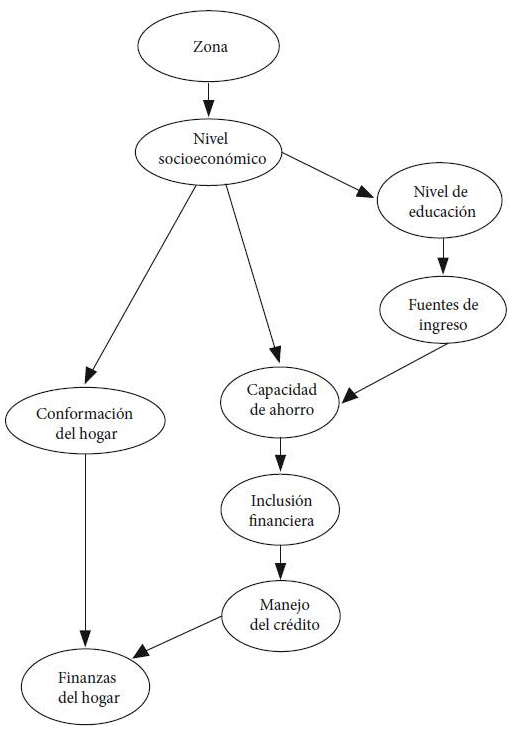
\includegraphics[width=6cm, height=7cm]{figuras/RD2.PNG}
\caption{Modelográfico de la red bayesiana de las finanzas del hogar.}
\label{RB2} 
\end{center}
\end{figure}

\begin{figure}[H]
\begin{center}
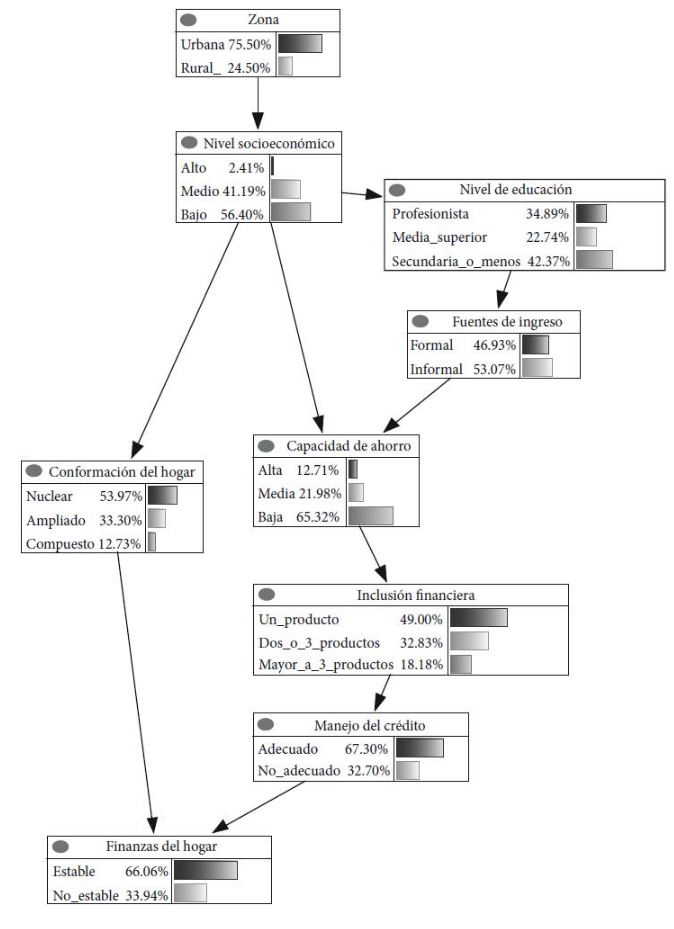
\includegraphics[width=8.5cm, height=8cm]{figuras/RB22.PNG}
\caption{Escenario: modelo gráfico de la Red Bayesiana con probabilidades.}
\label{RB22} 
\end{center}
\end{figure}

Una vez que los jefes del hogar tienen acceso al crédito: consumo, hipoteca, automotriz, concientizarlos acerca de la importancia de no incurrir en morosidad y mantener un buen historial crediticio se logra con educación financiera. Así, ceteris paribus, de todas las variables excepto manejo del crédito, se ejecuta el modelo, los resultados muestran que un manejo adecuado del crédito $(100\%)$ genera un incremento de $14\%$ en la probabilidad de FH estables respecto al estado base, es decir $80\%$ de probabilidad de FH estables, véase la Figura ~\ref{RB22}.

\textbf{\underline{Importancia:}}
En la investigación, las RB proporcionan una forma simple, rápida y eficiente para analizar los diferentes escenarios en el estudio del comportamiento de las finanzas de los hogares en México, cuyos resultados y análisis permiten inferir que es imprescindible promover políticas públicas que se enfoquen en complementar al currículo escolar e incorporen la impartición de educación financiera en todos los niveles y modalidades educativos; para el manejo adecuado de los créditos y la actividad financiera.

%--------------------------------------------------------------
\item En la tesis titulada \textit{\textbf{“Sistema experto probabilístico basado en redes bayesianas para la predicción de riesgo de cáncer cervical”}}, \citep{paulino2019sistema}, se realizó la predicción de riesgo de cáncer de cuello uterino usando un modelo probabilístico basado en Redes Bayesianas.\par
\textbf{\underline{Problema:}}
Los resultados estadísticos presentados por la OMS calculan que en el 2012 hubo 530,000 nuevos casos de cáncer de cuello uterino, los cuales representaron el 7.5\% de la mortalidad femenina, siendo la falta de prevención la principal causa.
En los países menos desarrollados la realidad es que se carecen de sistema de salud eficaces y de recursos financieros suficientes en comparación con los países desarrollados. En los países subdesarrollados no se cuenta con el personal capacitado para realizar el análisis respectivo y entregar el diagnóstico al paciente. Esto provoca retrasos en la entrega de resultados y genera pérdida de interés en los pacientes. \par
\textbf{\underline{Resultados:}}
Se implementó un sistema probabilístico basado en Redes Bayesianas (Ver Figura  ~\ref{R33} ) capaz de clasificar con una tasa de éxito de 96\% a personas diagnosticadas con cáncer de cuello uterino. Además de ello, gracias a la versatilidad y transparencia que ofrecen las Redes Bayesianas, se puede analizar las probabilidades de cada una de las variables.  Donde de un total de 322 registros se pudo
obtener 15 atributos o características diferentes que correspondan a la información de una
paciente. Las pruebas fueron realizadas utilizando el 40\% de los datos. Los resultados le
otorgan al trabajo desarrollado una tasa de éxito del 96\%.\par

\begin{figure}[H]
\begin{center}
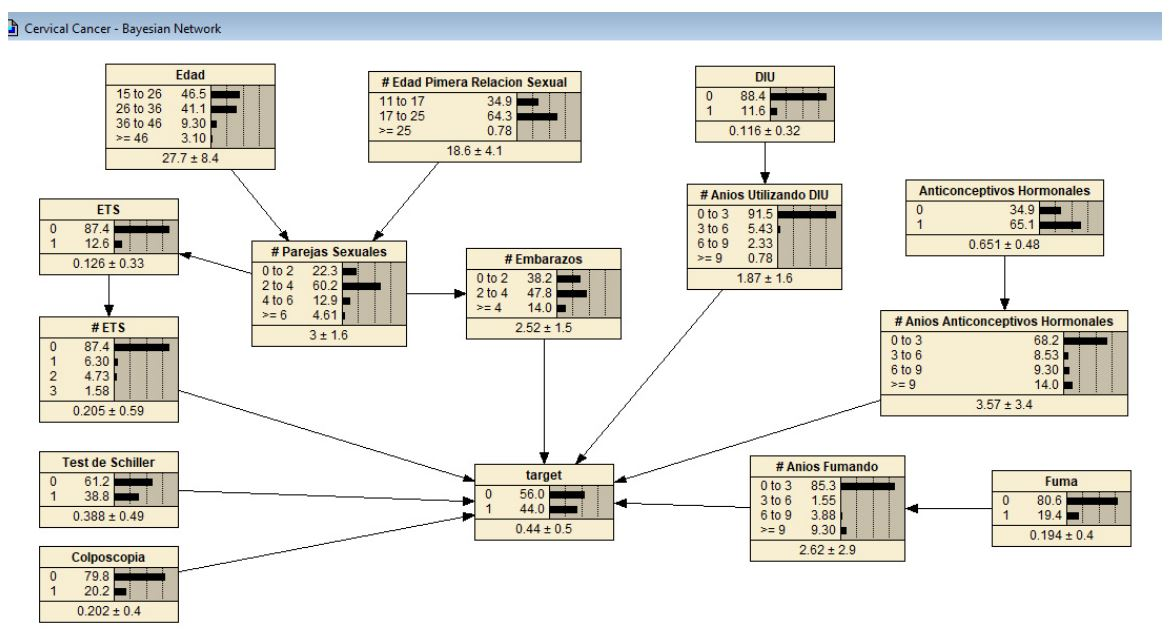
\includegraphics[width=8.7cm, height=7cm]{figuras/R33.JPG}
\caption{Estado de los nodos de la Red Bayesiana luego del Aprendizaje Paramétrico.}
\label{R33} 
\end{center}
\end{figure}

\textbf{\underline{Importancia:}}
El modelo probabilístico propuesto maximiza la cantidad de verdaderos positivos alcanzando una taza del 98\% al momento de identificar pacientes con riesgo de cáncer, esto es muy importante sobre todo dentro del área de dominio de la Medicina, ya que cometer un error al predecir un caso verdadero negativo no tiene el mismo impacto que comeré un error al predecir un caso verdadero positivo, es por ello que siempre se busca minimizar esto último, algo que el modelo propuesto basado en Redes Bayesianas logra al maximizar la eficiencia de identificar verdaderos positivos. \par

%--------------------------------------------------------------
\item Otra investigación es la tesis titulada \textit{\textbf{“Modelo Hidrológico de Predicción de Caudales de Avenida mediante Redes Bayesianas en la subcuenca del río Shullcas en el 2016”}}, \citep{gonzales2021modelo}, donde se realizó el desarrollo de un modelo hidrológico de predicción
de caudales de avenida construido a partir de las características geomorfológicas y datos hidrometeorológicos de la cuenca y posteriormente validado a través de las redes bayesianas.
\textbf{\underline{Problema:}}
Los caudales a diferencia de los demás elementos del ciclo hidrológico influyen con mayores consecuencias sobre la vida del ser humano, sirve como fuente primaria para diferentes usos, consumo doméstico, agricultura, industria, comercio, generación de electricidad, etc.
En este contexto la predicción de caudales surge a partir de la necesidad de conocer el período de anticipación máximo posible para que los beneficiarios adopten medidas que les permitan mitigar las pérdidas u optimizar las decisiones de gestión hídrica, tal es el caso del diseño de obras hidráulicas, ya que, por la falta de información proporcionada por las estaciones meteorológicas, puede hacer que una estructura este sobredimensionada o sobrevalorada.\par
\textbf{\underline{Resultados:}}
Para hacer uso de las redes bayesianas fue necesario estructurar las redes con variables que son suministradas por el modelo HBV, las cuales después de un proceso de correlación sirvieron para definir las estructuras de las dos redes bayesianas a utilizar, de las cuales se eligió la que tuvo menor error. Las redes bayesianas trabajaron con un grupo de datos discretizados y clasificados, luego de obtener la base de datos que usaron a través del programa NETICA se procedió a crear nodos y conexiones entre las variables intervinientes para poder tener las probabilidades a posteriori. Para el aprendizaje de las redes bayesianas se usaron el 70\% de datos totales y luego para su validación el otro 30\% de los casos. Para tener una evidencia de validez se observa la tasa de error de la misma, en este caso la red bayesiana N°2 presento un menor error de predicción que la red bayesiana N°1.
\par
\begin{figure}[H]
\begin{center}
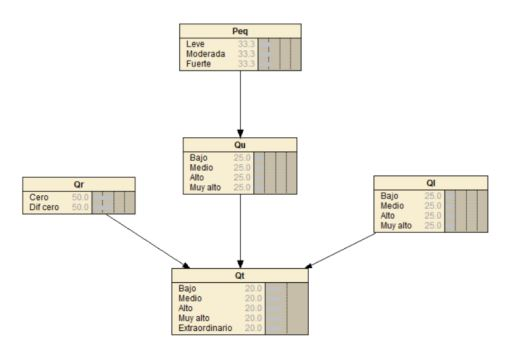
\includegraphics[width=8cm, height=6cm]{figuras/R34.JPG}
\caption{Topología de red bayesiana N°1 tras haber definido sus nodos y estados.}
\label{R34} 
\end{center}
\end{figure}

\begin{figure}[H]
\begin{center}
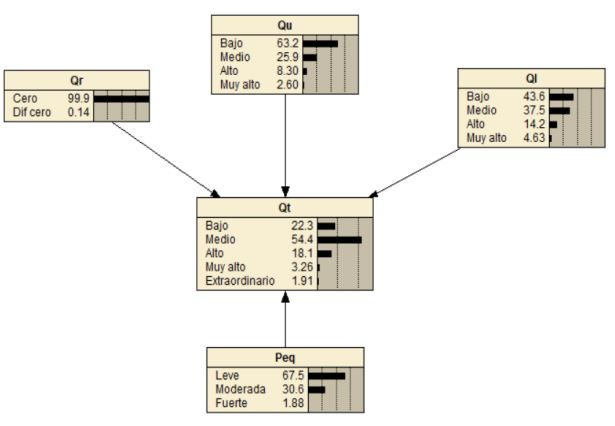
\includegraphics[width=8cm, height=6cm]{figuras/R35.JPG}
\caption{Topología de red bayesiana N°2 compilada.}
\label{R35} 
\end{center}
\end{figure}

\textbf{\underline{Importancia:}}
En la tesis se aplicó la topología para construir un modelo hidrológico para la cual se tomó diferentes valores para los parámetros de la cuenca (precipitación, parámetros morfológicos, usos de suelo), toda esta cantidad de datos
será tratada y nos ayudará a representar los procesos de transporte de caudal, teniendo
en cuenta asimismo las características de cada subcuenca y cauce considerado usando redes bayesianas.\par
\end{enumerate} 
%---------------------------------------------------------------------------
\section{\textbf{Conclusiones}}
Este informe presentó información relevante acerca de Redes Bayesianas empleadas en la Inteligencia Artificial, explicándose también los conceptos teóricos relacionados a ellas. Además de permitir conocer sobre algunas investigaciones que se vienen realizando año a año, entendiendo las diversas aplicaciones en la vida diaria. Concluimos que la mayoría analiza la problemática y dependiendo de sus características se estableció el análisis y proceso para representar o modelar la información y su incertidumbre o probabilidad. Finalmente, las investigaciones expuestas en este trabajo de recopilación, sirven como antecedentes y base a futuros investigadores a nivel nacional e internacional, que pueden ser usados tanto en el área comercial o académico.
%-------------------------------------------------------
\medskip
\bibliography{refer}
\end{document}